\documentclass[10pt]{beamer}

\usetheme[progressbar=frametitle,block=fill,background=light]{metropolis}
\usefonttheme{serif}

\usepackage{appendixnumberbeamer}

\usepackage{booktabs}
\usepackage[scale=2]{ccicons}


\usepackage{pgfplots}
\usepgfplotslibrary{dateplot}
\usepackage{pgfplotsthemetol}
\usepackage{amsmath,amssymb,amsthm,amsfonts,amstext}
\usepackage{bbm}

\usepackage{xspace}

\usepackage{import}
\import{}{Packages/custom_macros.tex}

\newcommand{\themename}{\textbf{\textsc{metropolis}}\xspace}
\renewcommand{\emph}{\alert}

\title{Group theory, Topology and Spin-$1/2$ Particles}
\subtitle{From Dirac's belt to fermions}
% \date{\today}
\date{}
\author{Louan Mol}
\institute{Unversité Libre de Bruxelles\\[2cm]{\small Brussels Summer School of Mathematics 2022}}
% \titlegraphic{\hfill\includegraphics[height=1.5cm]{logo.pdf}}

\begin{document}

\maketitle

\begin{frame}{Table of contents}
    \setbeamertemplate{section in toc}[sections numbered]
    \tableofcontents%[hideallsubsections]
\end{frame}

\section{Dirac's belt trick and rotations}

\begin{frame}{Dirac's belt trick}
    
    \visible<1->{
    You need:
    \begin{itemize}
      \item a belt (not necessarily Dirac's)
      \item a heavy book
    \end{itemize}
    Rules:
    \begin{enumerate}
      \item you can only move the end of the belt
      \item you cannot twist or rotate it
    \end{enumerate}
    \textbf{Goal:} untwist a $2\pi$-twist.\\[0.5cm]}

    \visible<2->{
      $\Rightarrow$ it tuns out to be \emph{impossible} ! One turn negates the twist: $2\pi\to-2\pi$. \\[0.5cm]
    }
    \visible<3->{
      Therefore, possible for a $4\pi$ twist ...\\ \hspace{7cm} Why is that ?
    }

\end{frame}

\begin{frame}{Space of rotations: $\SO(3)$ as a group}
      
      Rotations in $3$-dimensional space: matrices that acts on $\R^3$ and that \emph{preserve the scalar product}, and in particular \emph{lengths}.\\[0.3cm]
      In other words: matrix $O$ such that $O^TO=\mathbbm{1}$ ($\Leftrightarrow$ $O$ is orthogonal)\\[0.3cm]
      Additional requirement: orientation preserving $\Leftrightarrow$ $\det O=1$\\[0.3cm]

      \begin{block}{Special othogonal group}
        $\SO(3)$ is the set of $3\times 3$ real matrices such that $O^TO=\mathbbm{1}$ and $\det O=1$.
      \end{block}
      Three ``fundamental'' rotations:
      \begin{equation*}
        {\tiny
        x:
        \begin{bmatrix}
          1 & 0 & 0 \\
          0 & \cos\theta & -\sin\theta \\
          0 & \sin\theta & \cos\theta
        \end{bmatrix}\qquad
        y:
        \begin{bmatrix}
          \cos\theta & 0 & -\sin\theta \\
          0 & 1 & 0 \\
          \sin\theta & 0 & \cos\theta
        \end{bmatrix}\qquad
        z:
        \begin{bmatrix}
          \cos\theta & -\sin\theta & 0 \\
          \sin\theta & \cos\theta & 0 \\
          0 & 0 & 1
        \end{bmatrix}}
      \end{equation*}

      $\Rightarrow$ It forms a \emph{group}.
    
\end{frame}

\begin{frame}{Space of rotations: $\SO(3)$ as a topological space}
  
\end{frame}



\begin{frame}
  The belt trick is a way of physically demonstrating the the fundamental group of $\SO(3)$ is $\Z_2$.
\end{frame}

% How is that useful ?

\begin{frame}{Electrons}
  \visible<1->{
    In quantum mechanics
  }
\end{frame}

\begin{frame}

    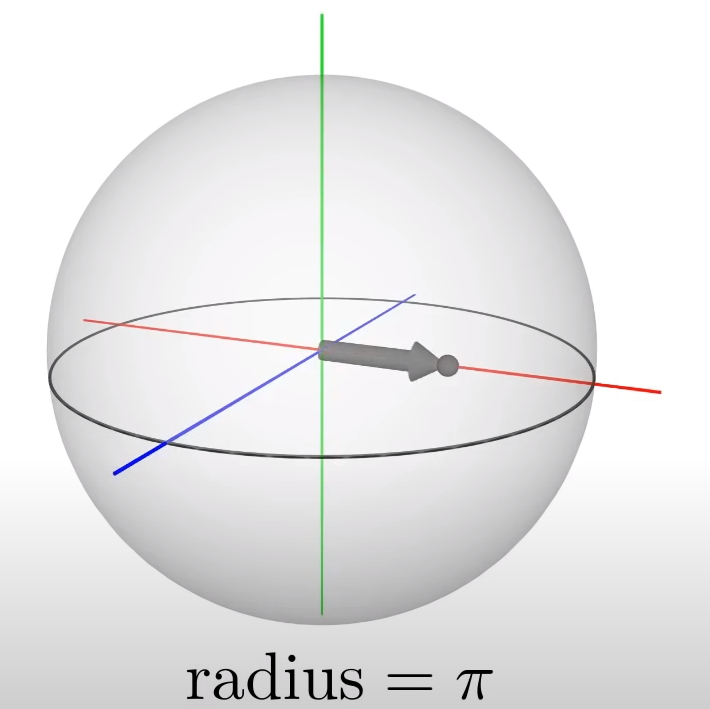
\includegraphics[scale=0.1]{Pictures/SO3sphere.png}

    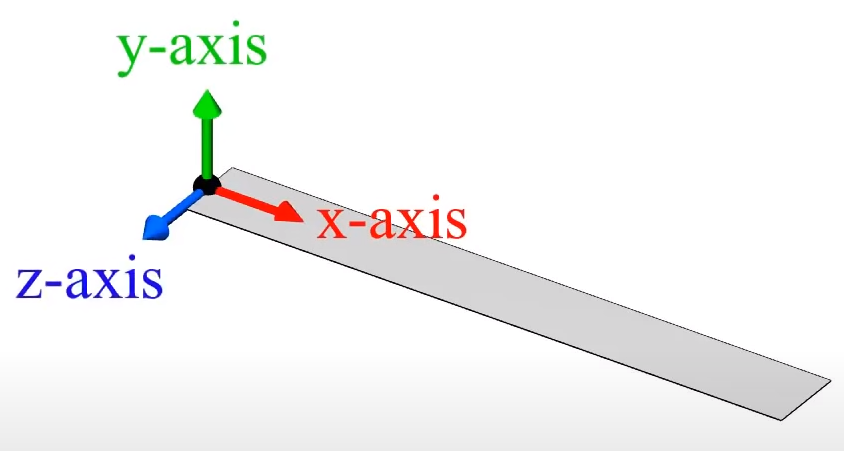
\includegraphics[scale=0.1]{Pictures/beltaxis.png}

    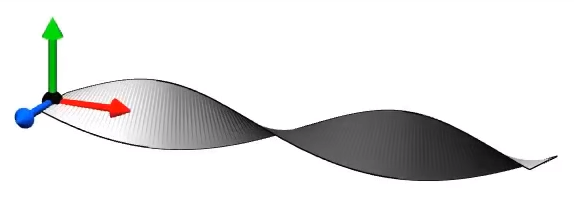
\includegraphics[scale=0.1]{Pictures/xaxisbelt.png}

    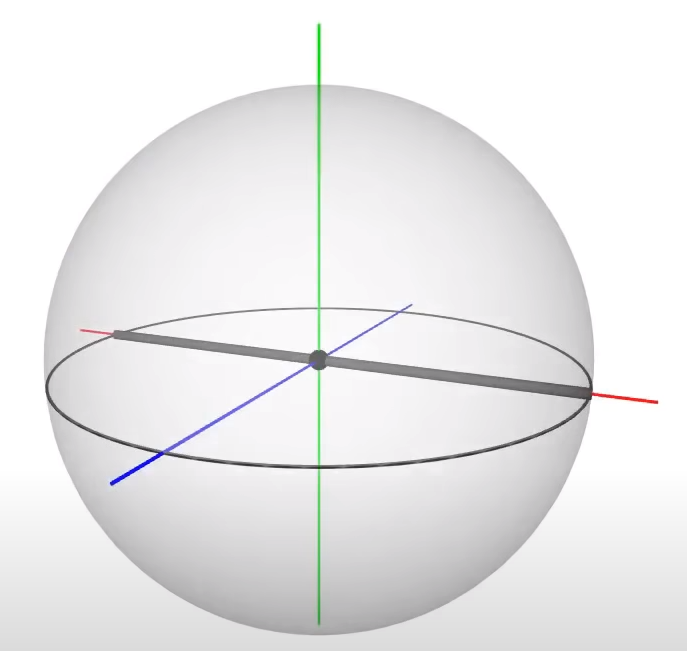
\includegraphics[scale=0.1]{Pictures/xaxissphere.png}

    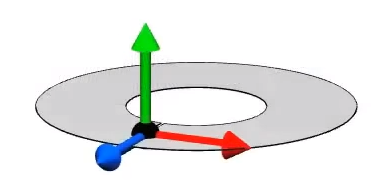
\includegraphics[scale=0.1]{Pictures/yaxisbelt.png}

    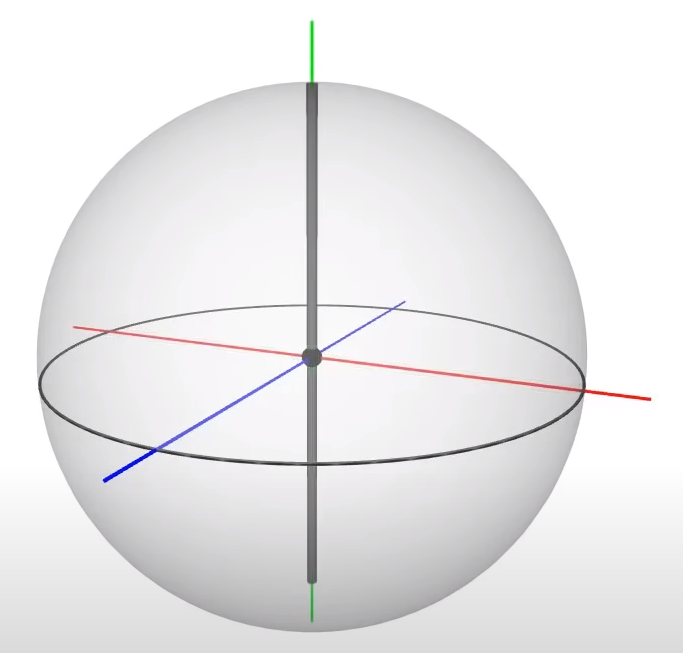
\includegraphics[scale=0.1]{Pictures/yaxissphere.png}

    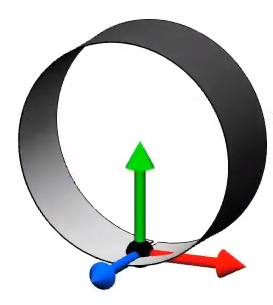
\includegraphics[scale=0.1]{Pictures/zaxisbelt.png}

    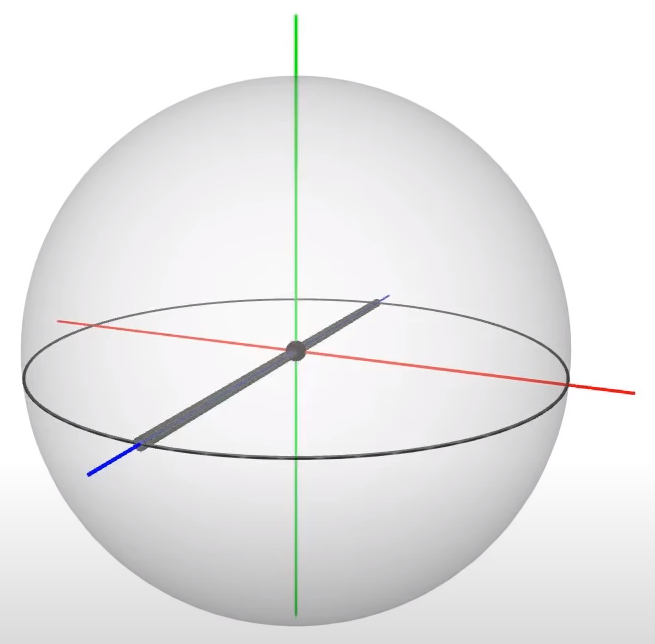
\includegraphics[scale=0.1]{Pictures/zaxissphere.png}

    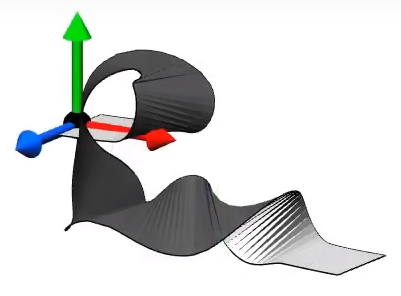
\includegraphics[scale=0.1]{Pictures/randomrotbelt.png}

    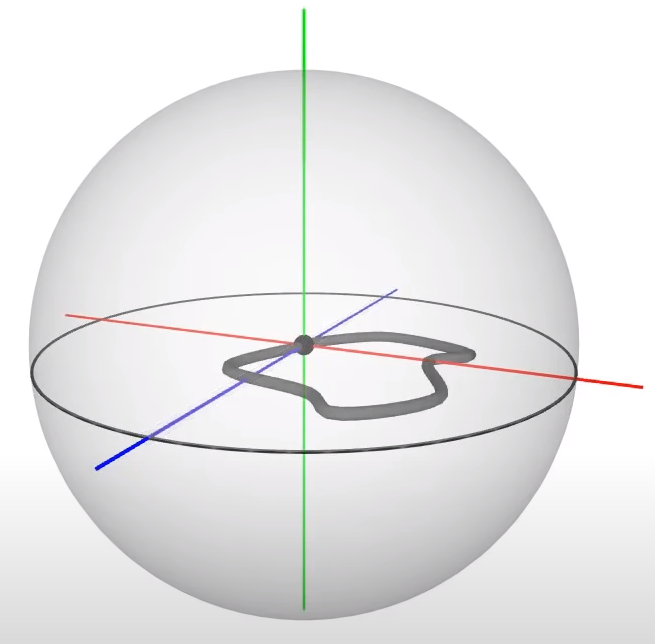
\includegraphics[scale=0.1]{Pictures/randomrotsphere.png}

    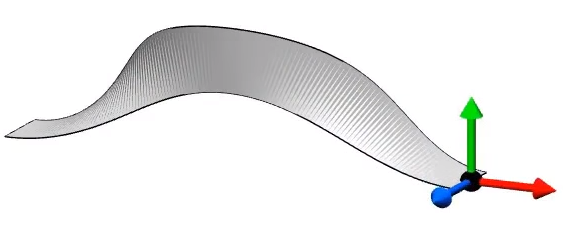
\includegraphics[scale=0.1]{Pictures/contractiblepathbelt.png}

    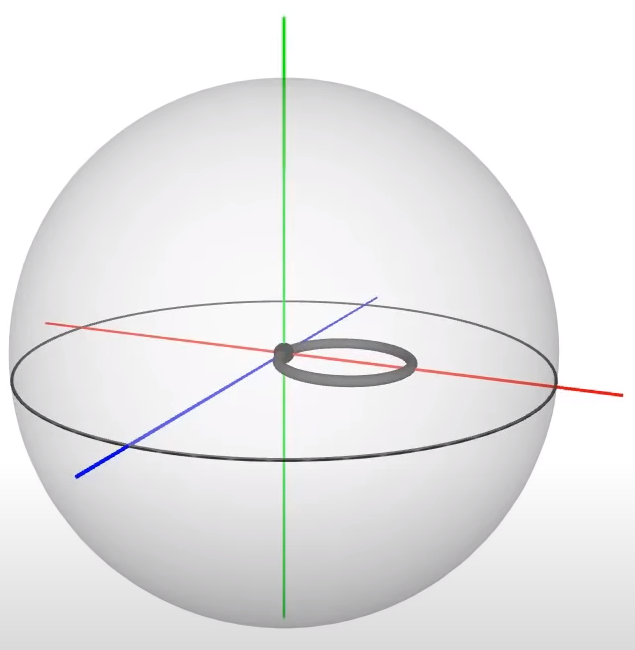
\includegraphics[scale=0.1]{Pictures/contractiblepathsphere.png}

    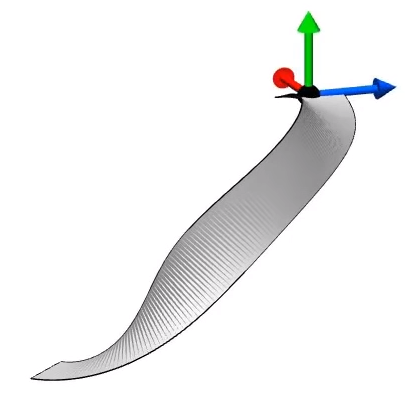
\includegraphics[scale=0.1]{Pictures/noncontractiblepathbelt.png}

    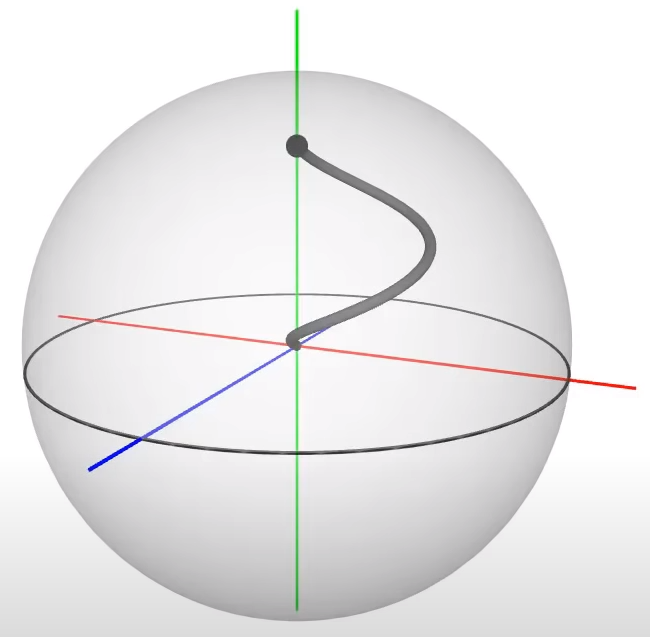
\includegraphics[scale=0.1]{Pictures/noncontractiblepathsphere.png}

    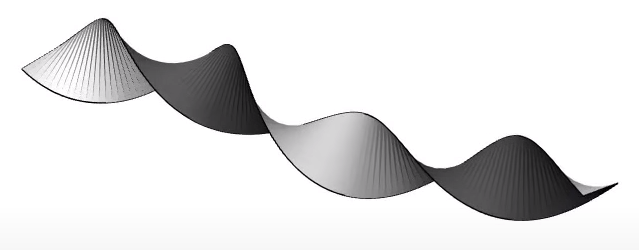
\includegraphics[scale=0.1]{Pictures/4pibelt.png}

    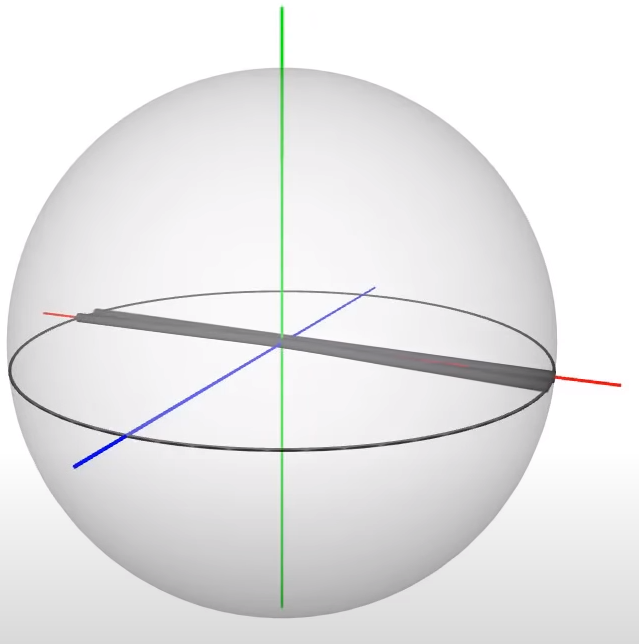
\includegraphics[scale=0.1]{Pictures/4pisphere1.png}

    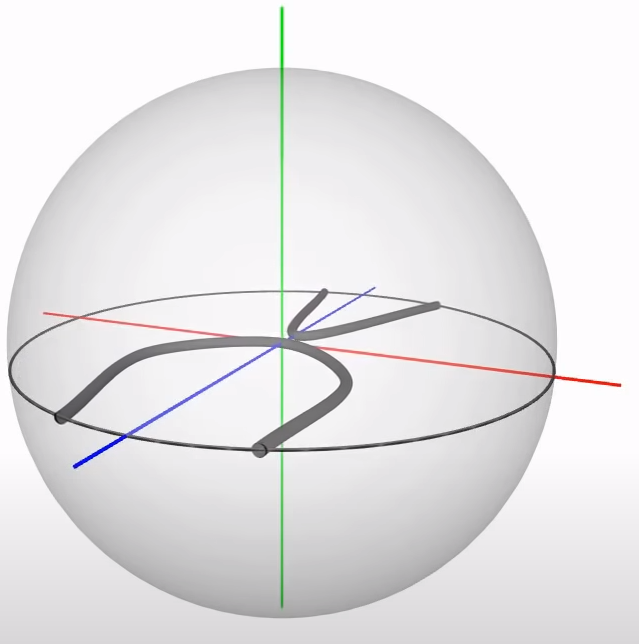
\includegraphics[scale=0.1]{Pictures/4pisphere2.png}

    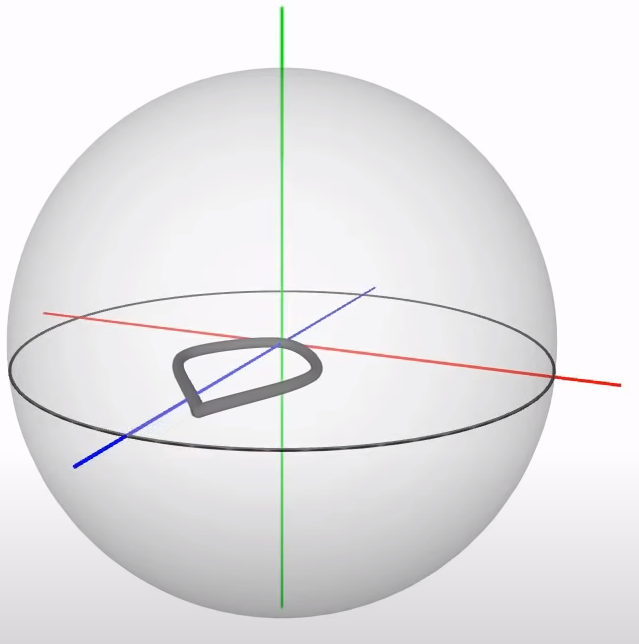
\includegraphics[scale=0.1]{Pictures/4pisphere3.png}

    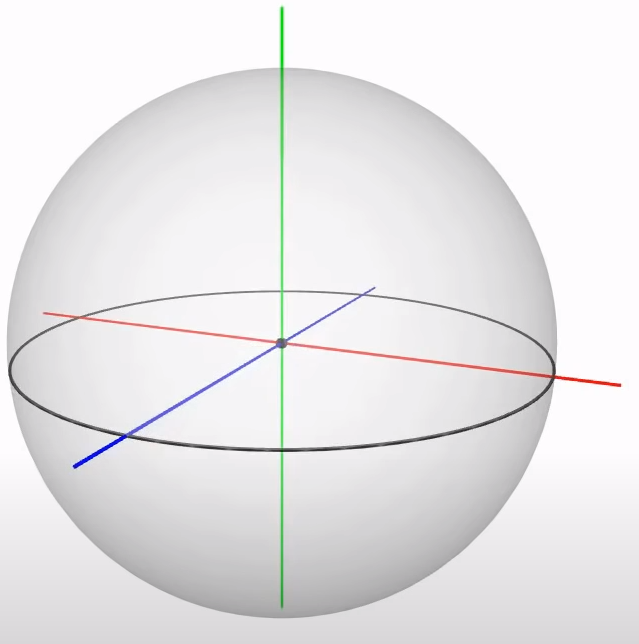
\includegraphics[scale=0.1]{Pictures/4pisphere4.png}

    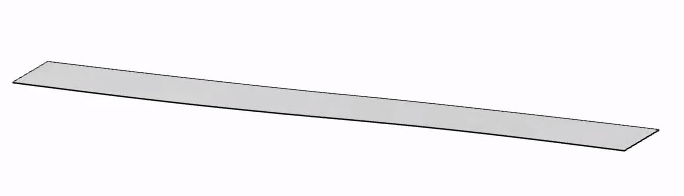
\includegraphics[scale=0.1]{Pictures/flatbelt.png}

\end{frame}

\section{Section 2}

\section{Section 3}

\section{Section 4}

\section{Section 5}

\begin{frame}{Blocks}
    Three different block environments are pre-defined and may be styled with an
    optional background color.
  
    \begin{columns}[T,onlytextwidth]
        \column{0.5\textwidth}
          
            Some text.\\[2cm]
            aaaaa
    
        \column{0.5\textwidth}
    
          \begin{block}{Default}
            Block content.
          \end{block}
    
          \begin{alertblock}{Alert}
            Block content.
          \end{alertblock}
    
          \begin{exampleblock}{Example}
            Block content.
          \end{exampleblock}
    
      \end{columns}

  \end{frame}

\appendix

\begin{frame}[fragile]{Backup slides}
  Sometimes, it is useful to add slides at the end of your presentation to
  refer to during audience questions.

  The best way to do this is to include the \verb|appendixnumberbeamer|
  package in your preamble and call \verb|\appendix| before your backup slides.

  \themename will automatically turn off slide numbering and progress bars for
  slides in the appendix.  \cite{ConcreteMath}
\end{frame}

\begin{frame}[allowframebreaks]{References}

  \bibliography{bibliography}
  \bibliographystyle{abbrv}

\end{frame}

\end{document}
